%
% tp 2 mna
% 

% Use emulateapj instead to make Apj format.
% YOU SHOULD REMOVE THE TABLE OF
% CONTENTS PAGE WHEN USING APJ FORMAT.
\documentclass[11pt,a4paper]{emulateapj}
\bibliographystyle{apj}


%define general packages
\usepackage{epsfig}
\usepackage{amsmath}
\usepackage{natbib}

% spanish packages
\usepackage[utf8]{inputenc}
\usepackage[spanish]{babel}
\languageshorthands{none}
\noextrasspanish
\let\layoutspanish\relax
\usepackage[spanish]{babel}
\renewcommand\shorthandsspanish{}

%internal short cuts
\def \HgA {H$\gamma_A$}
\def \gon {Gonz\'{a}lez}
\def \Hbp {H$\beta ^\prime$}
\def \warn {{\sffamily\bfseries\large WARNING, ARREGLAR:}}









\begin{document}

\submitted{Departamento Ing. en Informática, ITBA}
\title{Filtros espaciales en imagenes mediante el paso del dominio de los colores al dominio de las frecuencias}
\author{Williams M. \& Aráoz M.}
\date{\today}


\begin{abstract}
\warn{hacer abstract}
\end{abstract}

\maketitle




\section{Introduccción}
\label{sec:introduccion}

%\begin{figure*}
%  \begin{center}
%    \leavevmode
%      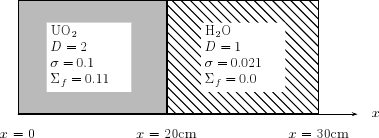
\psfig{file=images/img1.png, width=254px}
%       \caption[Esquema simple del reactor]{Modelo de un ractor nuclear unidimensional.
%         Diagrama adaptado de \citet{diaz10}.}
%     \label{fig:esquema}
%  \end{center}
%\end{figure*}


\section{Filtros utilizados}
\label{sec:sec2}
Para este trabajo utilizamos 3 filtros. El primero lo llamamos Pulso y cumple la esta definido por la siguiente función:

\begin{eqnarray}
H(k,l) = \left\{
	\begin{matrix}
		0, 0 \leq k \leq 400, 190 \leq l \leq 210 \\
		0, 0 \leq l \leq 400, 190 \leq k \leq 210 \\
		1, \quad $resto de las posiciones$
	\end{matrix} 
	\right.
\end{eqnarray}

El segundo filtro que utilizamos es el llamado Gaussiano:

\begin{eqnarray}
H(k,l) = e^{-0.1(k^2 + l^2)}
\end{eqnarray}
El filtro gaussiano lo que hace es aplicarle una difusión a la imagen. Es decir cambiando el valor por cual está multiplicado, la suma de los cuadrados de las variables, se puede variar la profundidad de la difusión. Es decir, al hacer ese valor más chico en valor absoluto, se logra una imagen menos difusa, pero al agrandar ese valor, la imagen obtenida se vuelve cada vez más difusa.
\\
El último filtro utilizado es el que llamamos Damero:
\begin{eqnarray}
H(k,l) = \left\{
	\begin{matrix}
		0,$ si $l+k$ es par$\\
		1,$ si $l+k$ es impar$\\
	\end{matrix} 
	\right.
\end{eqnarray}


\section{Seccion 3}
\label{sec:sec3}




\section{Resultados y Conclusiones}
\label{sec:resultadosyconclusiones}

%
\bibliography{paper}

\end{document}

